\documentclass{article}

\usepackage{graphicx}
\usepackage{tikz}
\usepackage{tikzsymbols}
\usetikzlibrary{calc,patterns,shapes.geometric}
\pagestyle{empty}
\usepackage[margin=0pt]{geometry}
\geometry{papersize={14in,12in}}

\def\centerarc[#1](#2)(#3:#4:#5){\draw[#1] ($(#2)+({#5*cos(#3)},{#5*sin(#3)})$) arc (#3:#4:#5);}

\begin{document}
	\begin{figure}
		\centering
		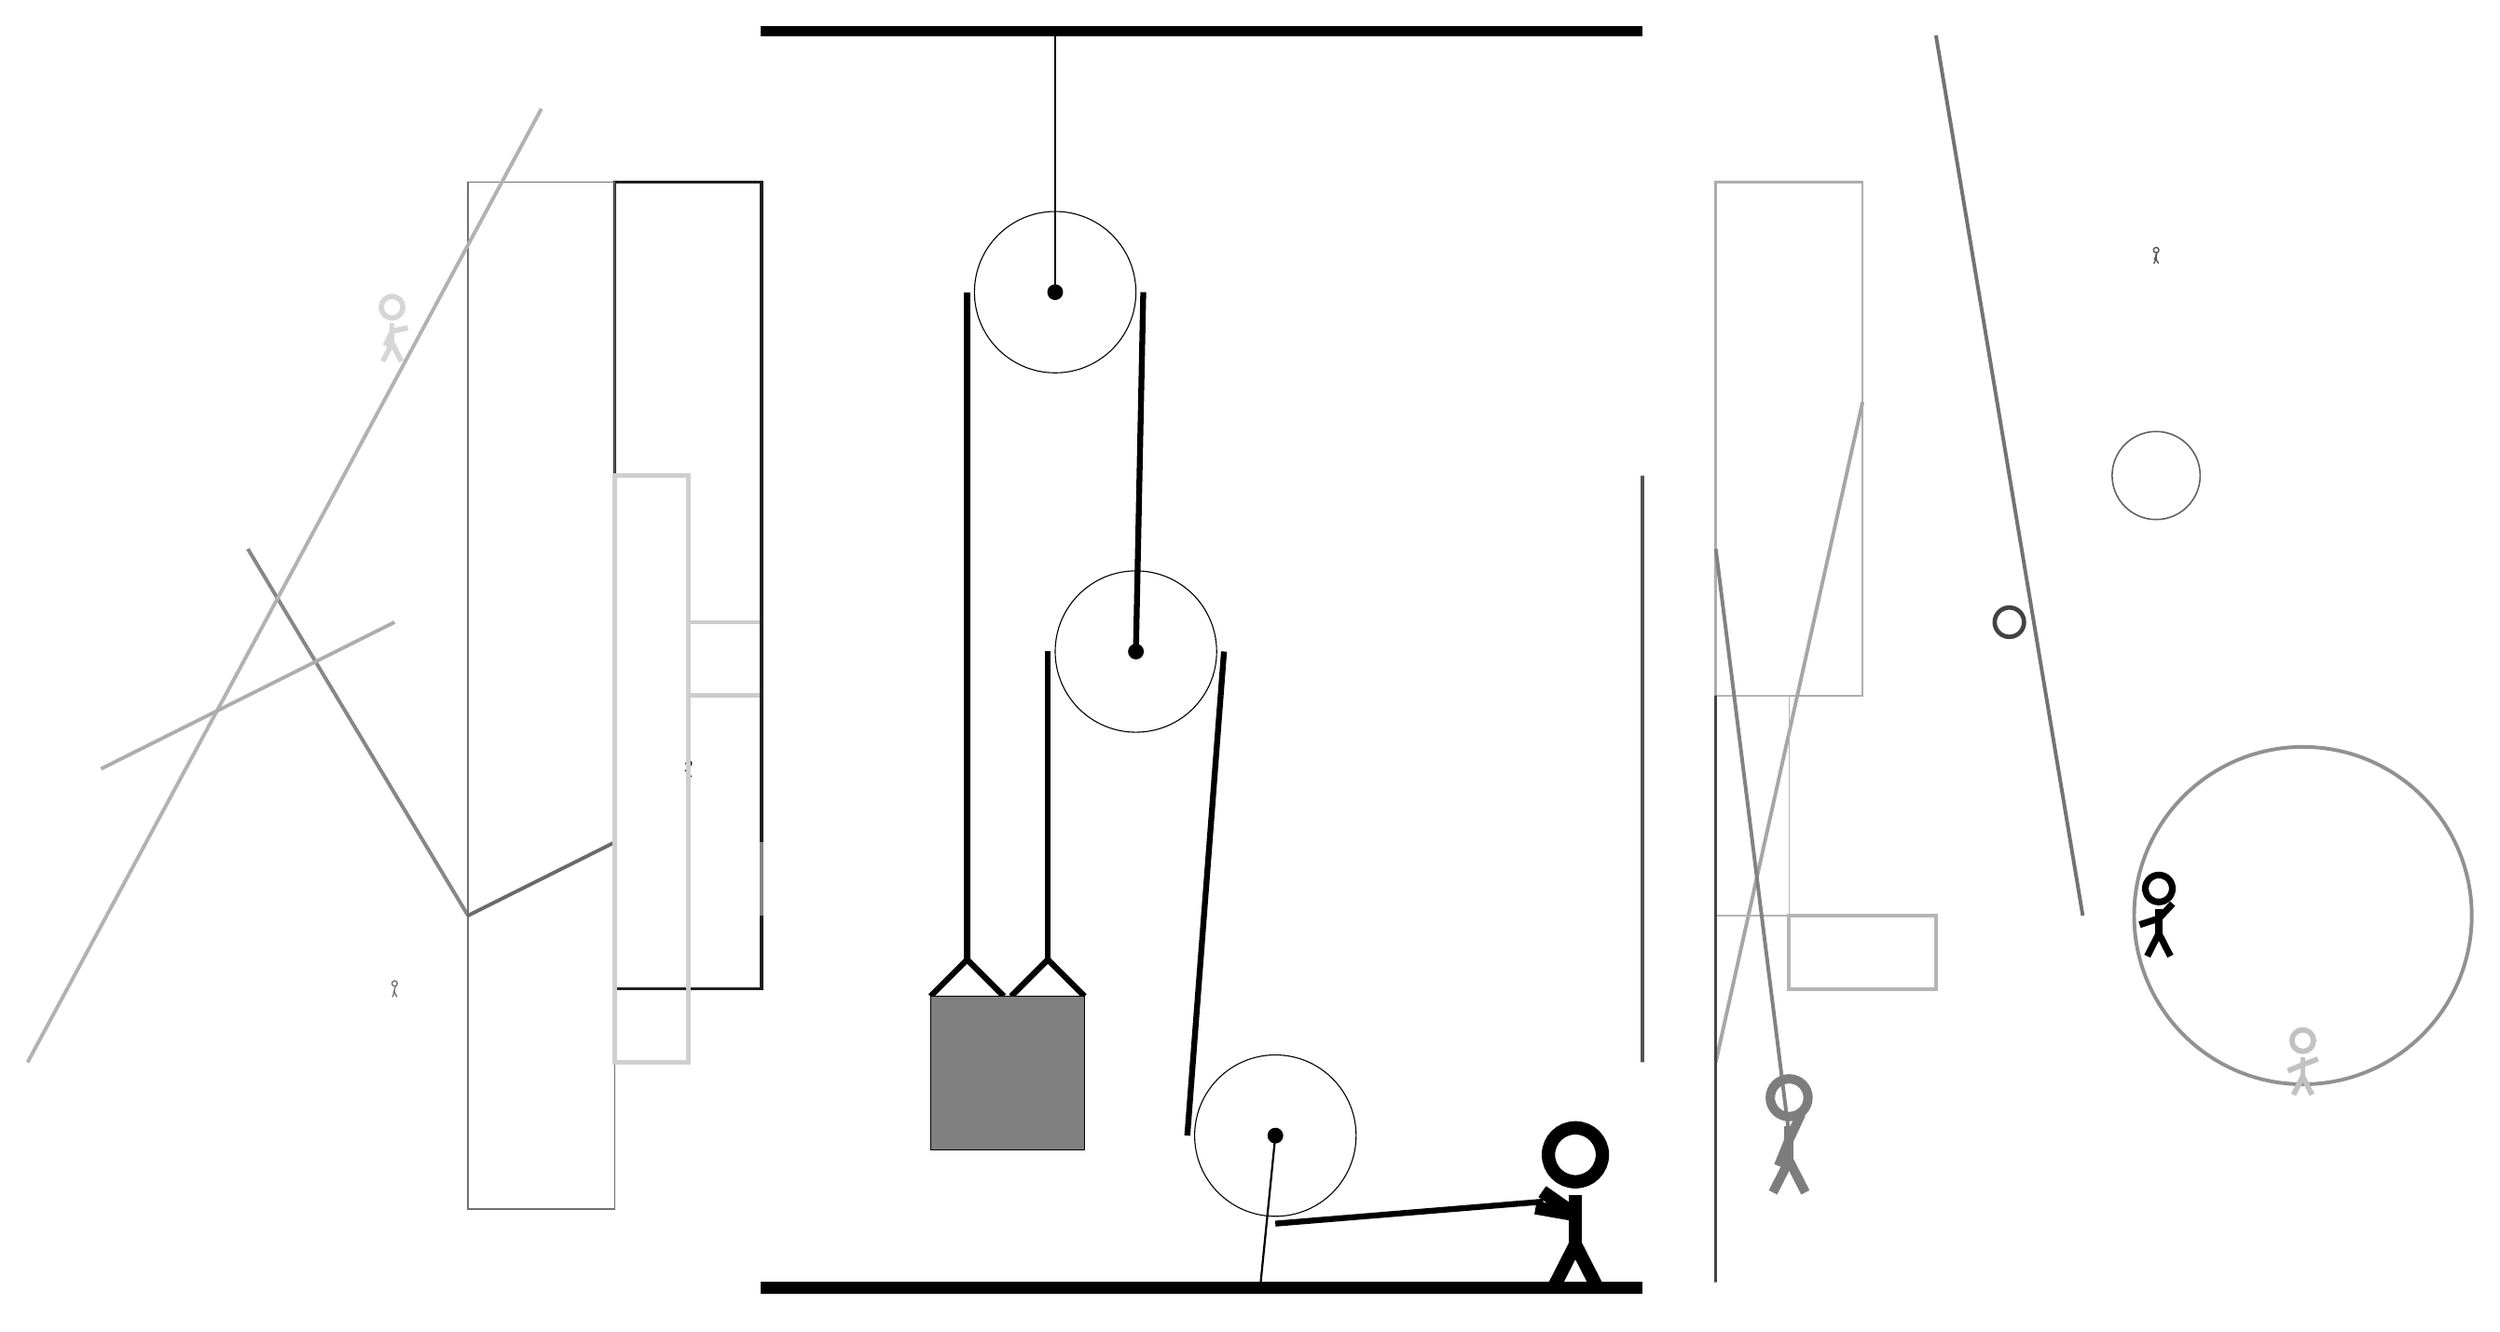
\begin{tikzpicture}
			%%%%% START %%%%%
			
			\draw[fill=black] (-2, 14) rectangle (10, 14.125);
			
			\node[line width=0.6mm, color=black!100] at (17, 2) {\Strichmaxerl[5][18][47]};
			
			\draw [line width=0.5mm, color=black!43](19, 2) circle (2.3);
			\draw[line width=0.3mm, color=black!32] (11, 12) rectangle (13, 5);
			\draw[line width=0.6mm, color=black!20] (-2, 5) rectangle (-3, 6);
			\draw[line width=0.5mm, color=black!35](11, 0) -- (13, 9);
			\node[line width=0.6mm, color=black!65] at (17, 11) {\Strichmaxerl[1][60][76]};
			\draw[line width=0.4mm, color=black!88] (-4, 12) rectangle (-2, 1);
			
			\draw[line width=0.5mm, color=black!47](-6, 2) -- (-9, 7);
			\draw[line width=0.2mm, color=black!56] (-4, 12) rectangle (-6, -2);
			\draw[line width=0.5mm, color=black!55](14, 14) -- (16, 2);
			\draw[line width=0.5mm, color=black!29] (12, 2) rectangle (14, 1);
			\draw [line width=0.2mm, color=black!62](17, 8) circle (0.6);
			\node[line width=0.7mm, color=black!16] at (-7, 10) {\Strichmaxerl[4][65][12]};
			
			\draw[line width=0.5mm, color=black!30](-5, 13) -- (-12, 0);
			\draw[line width=0.4mm, color=black!29] (-3, -2) rectangle (-3, -2);
			\draw[line width=0.2mm, color=black!58] (11, 1) rectangle (11, 1);
			\draw[line width=0.2mm, color=black!29] (12, 2) rectangle (11, 5);
			
			\draw[line width=0.5mm, color=black!49](11, 7) -- (12, -1);
			\draw[line width=0.5mm, color=black!67] (10, 8) rectangle (10, 0);
			\node[line width=0.4mm, color=black!53] at (-7, 1) {\Strichmaxerl[1][73][78]};
			\draw[line width=0.5mm, color=black!32](-7, 6) -- (-11, 4);
			\draw[line width=0.5mm, color=black!58](-6, 2) -- (-4, 3);
			\node[line width=0.7mm, color=black!24] at (19, 0) {\Strichmaxerl[4][23][20]};
			\draw[line width=0.5mm, color=black!48] (-2, 3) rectangle (-2, 2);
			\node[line width=0.4mm, color=black!51] at (12, -1) {\Strichmaxerl[7][68][65]};
			\draw [line width=0.6mm, color=black!74](15, 6) circle (0.2);
			\node[line width=0.3mm, color=black!96] at (-3, 4) {\Strichmaxerl[1][21][75]};
			\draw[line width=0.4mm, color=black!73] (11, 5) rectangle (11, -3);
			\draw[line width=0.6mm, color=black!19] (-3, 8) rectangle (-4, 0);
			
			
			\draw (2, 10.5) circle (1.1);
			\draw[fill=black] (2, 10.5) circle (0.1);
			\draw[thick] (2, 10.5) -- (2, 14);
			
			\draw (3.1, 5.6) circle (1.1);
			\draw[fill=black] (3.1, 5.6) circle (0.1);
			
			\draw (5, -1) circle (1.1);
			\draw[fill=black] (5, -1) circle (0.1);
			\draw[thick] (5, -1) -- (4.8, -3);
			
			\draw[line width = 0.8mm]  (0.3, 0.9) -- (0.8, 1.4) -- (1.3, 0.9);
			\draw[line width = 0.8mm]  (1.4, 0.9) -- (1.9, 1.4) -- (2.4, 0.9);
			\draw[fill=black!50] (0.3, 0.9) rectangle (2.4, -1.2);
			
			\draw[line width = 0.8mm] (0.8, 10.5) -- (0.8, 1.4);
			\centerarc[line width = 0.8mm](2, 10.5)(0:180:1.2000000000000002);
			\draw[line width = 0.8mm] (3.2, 10.5) -- (3.1, 5.6);
			\draw[line width = 0.8mm] (1.9, 5.6) -- (1.9, 1.4);
			\centerarc[line width = 0.8mm](3.1, 5.6)(0:180:1.2000000000000002);
			\draw[line width = 0.8mm] (4.3, 5.6) -- (3.8, -1);
			\centerarc[line width = 0.8mm](5, -1)(180:270:1.2000000000000002);
			\draw[line width = 0.8mm] (5, -2.2) -- (8.65, -1.9);
			
			\node at (9, -2) {\Strichmaxerl[10][-35][170]};
			
			\draw[fill=black] (-2, -3) rectangle (10, -3.15);
			
			%%%%% END %%%%%
		\end{tikzpicture}
	\end{figure}	
\end{document}